\begin{slide}{EXAFS Analysis: Second Shell of FeO}

  \begin{cenpage}{135mm}

  Adding the 2nd shell Fe -- {\file{feffNNNN.dat}} for Fe-Fe -- and
  refining {\Blue{${R}$}}, {\Blue{${N}$}}, {\Blue{${\sigma^2}$}}:

    \vspace{1mm}

    \begin{tabular}{ll}
      \begin{minipage}{65mm}
        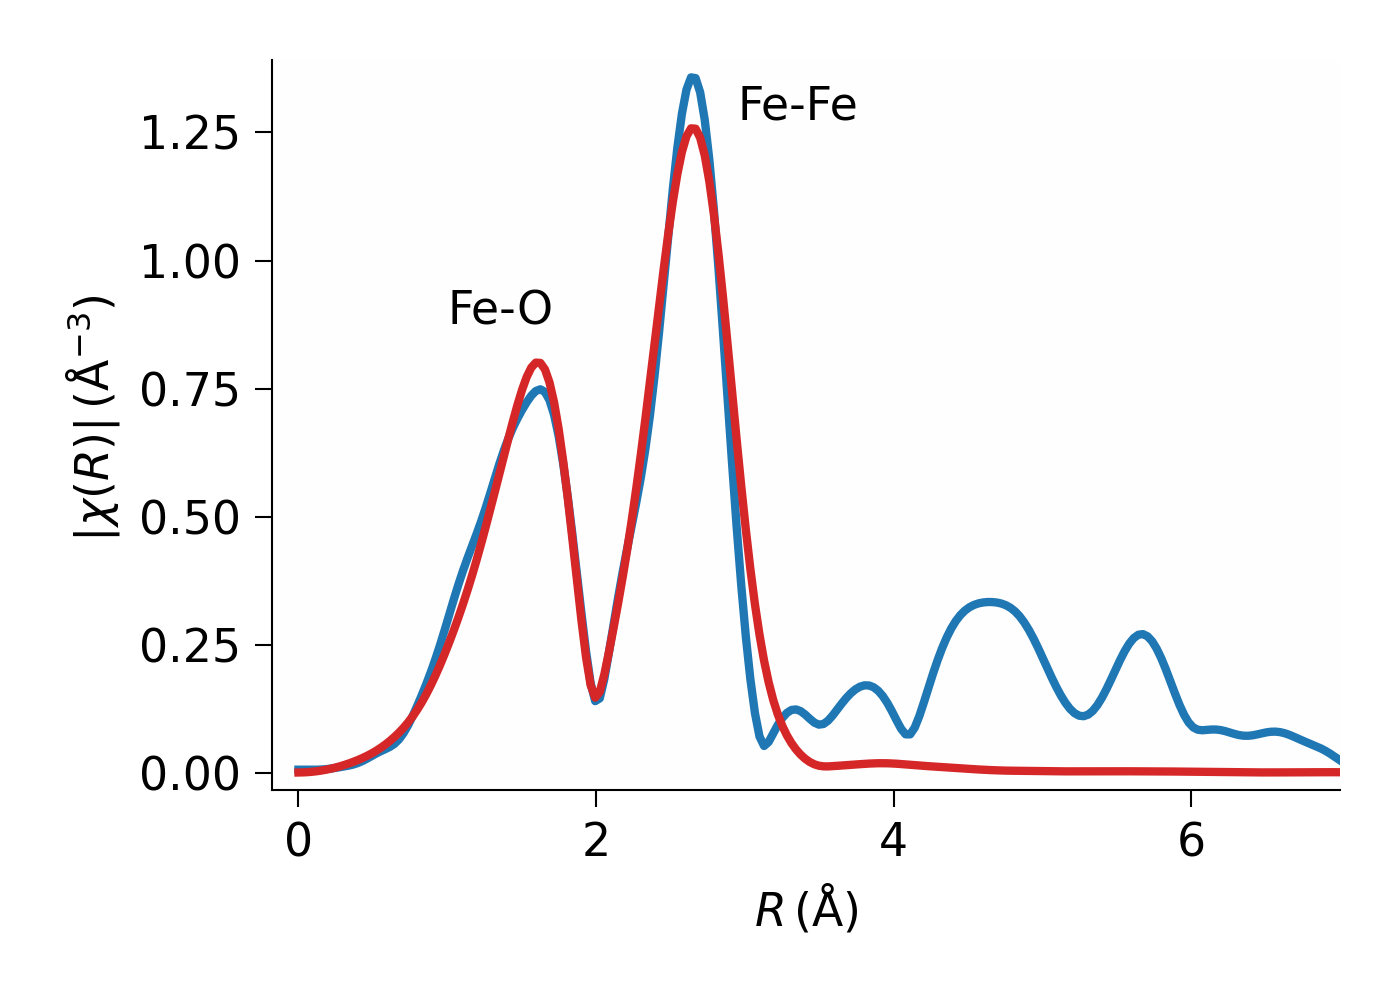
\includegraphics[width=63mm]{figs/fits/feo_2sh_chirmag}
      \end{minipage}
      &
      \begin{minipage}{49mm}
        \vspace{1mm}

        ${|\chi(R)|}$ data for FeO (blue), and fit of ${\rm
          1^{st}}$ and ${\rm 2^{nd}}$ shells (red).  \vfill
        \vspace{1mm}

        These
        results are consistent with the known values for FeO:\par
         6 O at 2.14\AA, 12 Fe at 3.03\AA.
    \end{minipage}
  \end{tabular}

  \onslide+<2->{
  Fit results:     \hspace{6mm} Statistics: $R \approx 0.01 $
 \hspace{5mm}  $\chi^2_\nu \approx 3 $.

  \begin{center}
    \begin{tabular}{|c|rrrr|}
    \hline
    Shell & ${N}$ & ${R}$ (\AA) & ${\sigma^2}$
    (${\rm\AA^2}$) & ${\Delta E_0}$ (eV) \\
    \hline
    Fe-O  &  4.6(0.6) & 2.11(.01) & 0.011(.002) & {\Red{1.8(0.7)}}\\
    Fe-Fe & 14.1(1.7) & 3.08(.01) & 0.015(.002) & {\Red{1.8(0.7)}}\\
    \hline
  \end{tabular}
  \end{center}

  \vmm

  }
  \onslide+<3-> {
  These are typical even for a ``very good fit'' on known structures.

  The calculation for ${{\Red{f(k)}}}$ and
  ${{\Red{\delta(k)}}}$ are good, but not perfect!
}

\end{cenpage}

\vfill
\end{slide}

\begin{slide}{EXAFS Analysis: Second Shell of FeO}

  \begin{cenpage}{135mm}

  Other views of the data and fit:

    \begin{tabular}{ll}
      \begin{minipage}{65mm}
        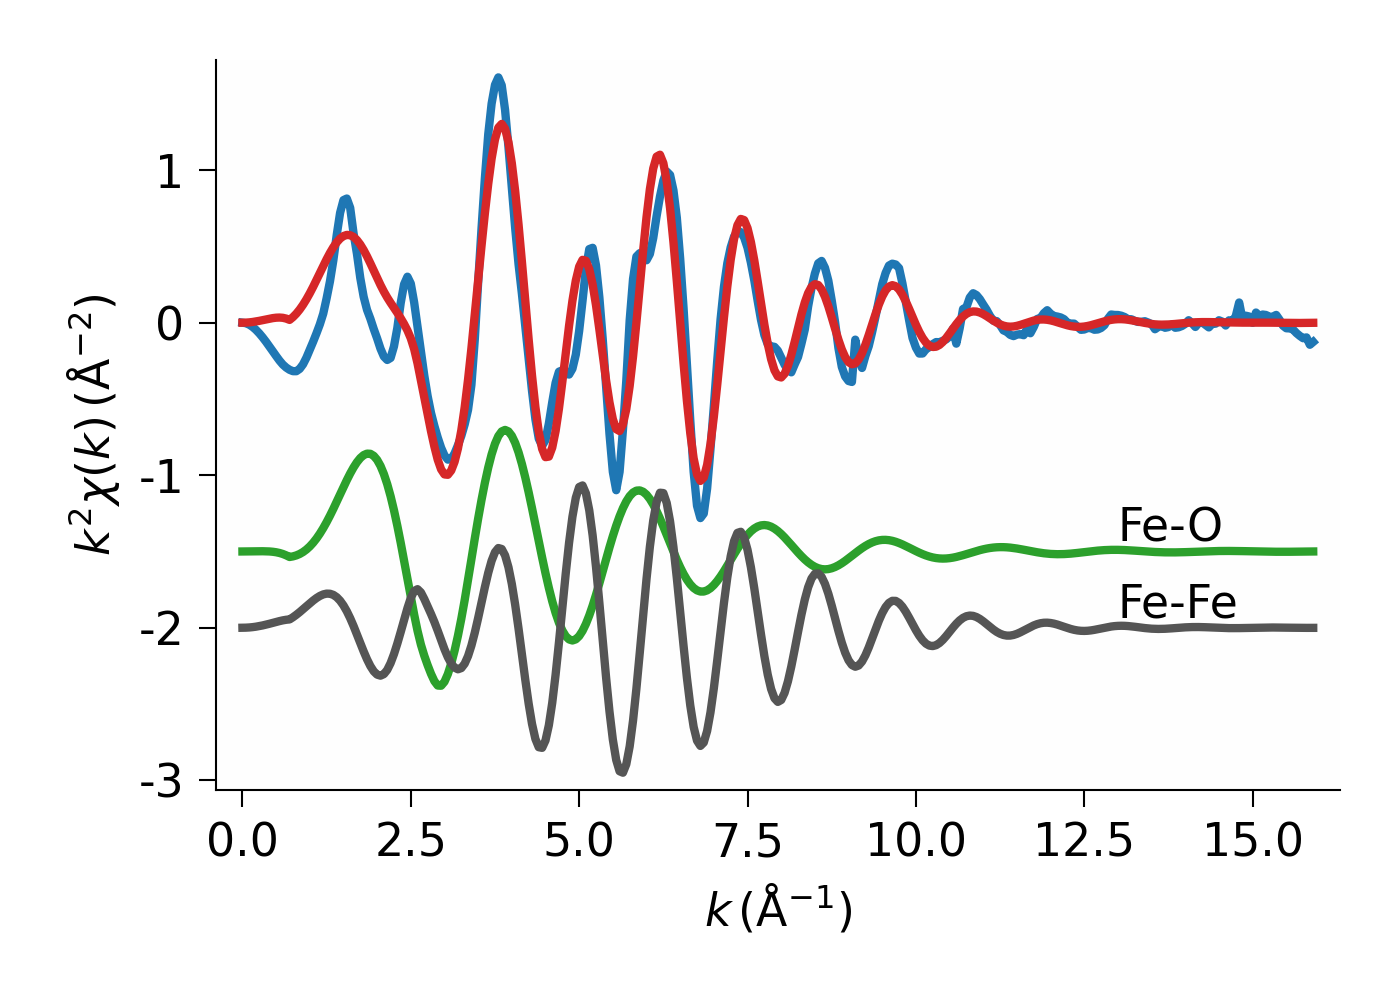
\includegraphics[width=60mm]{figs/fits/feo_2sh_chik}
      \end{minipage}
      &
      \begin{minipage}{65mm}  \setlength{\baselineskip}{11pt}
        The Fe-Fe EXAFS extends to higher-$k$ than the Fe-O EXAFS.

        \vmm Even in this simple system, there is some
        {\RedEmph{overlap}} of shells in ${R}$-space.

        {\onslide+<2->
          \vmm The fit in ${\rm Re[\chi(R)]}$ look especially
          good -- this is how the fits are done.

          \vmm
          }

    \end{minipage}
    \\
    \begin{minipage}{65mm}
        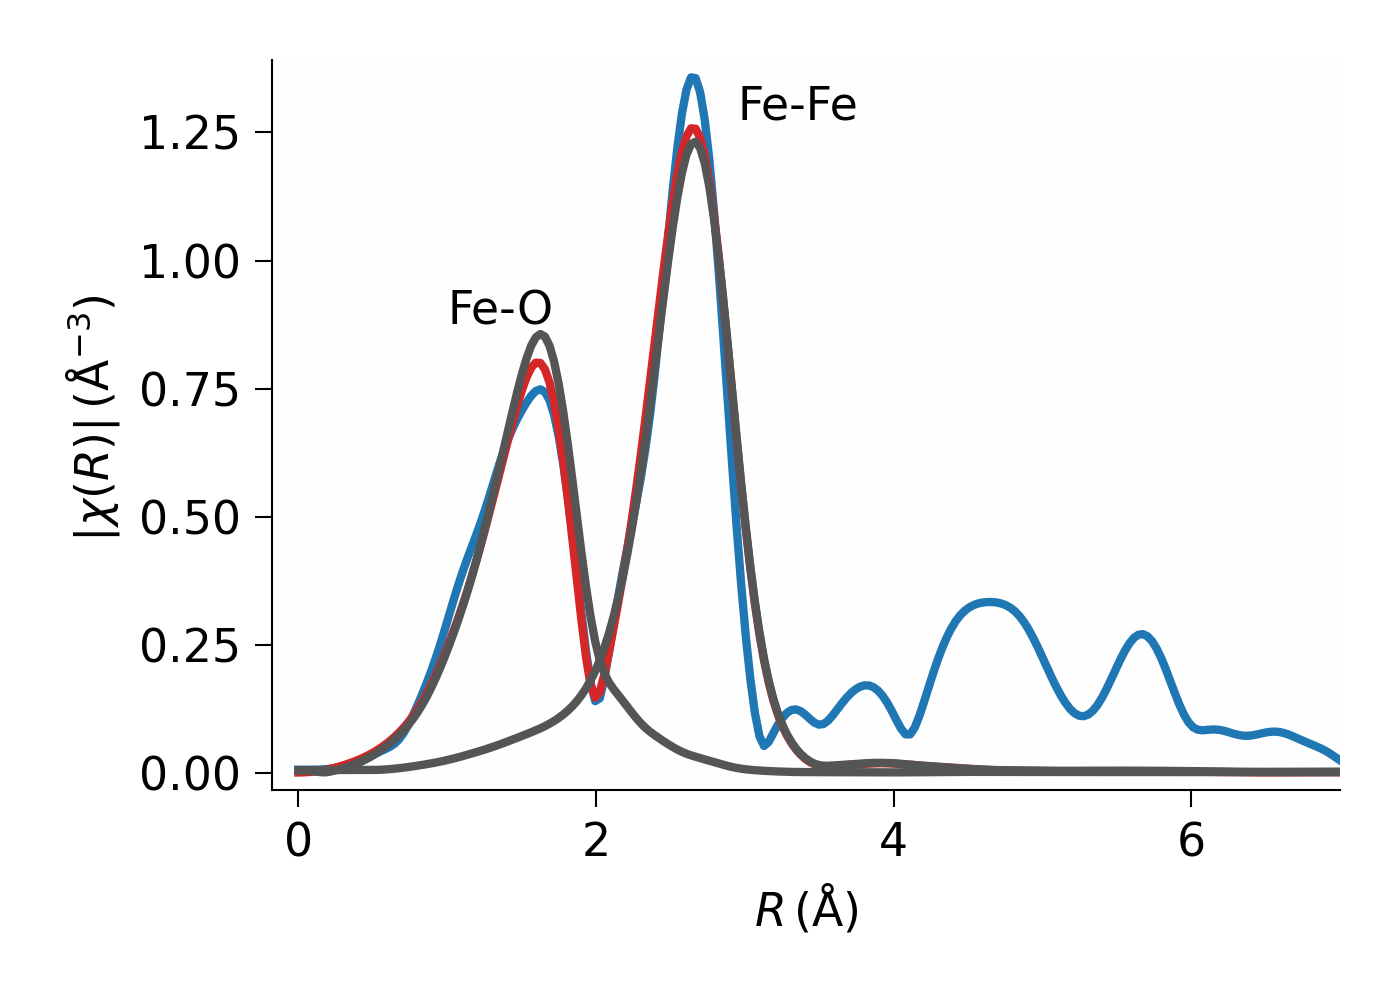
\includegraphics[width=60mm]{figs/fits/feo_2sh_chirmag_paths}
    \end{minipage}
    &
    \onslide+<2->{
      \begin{minipage}{65mm}
        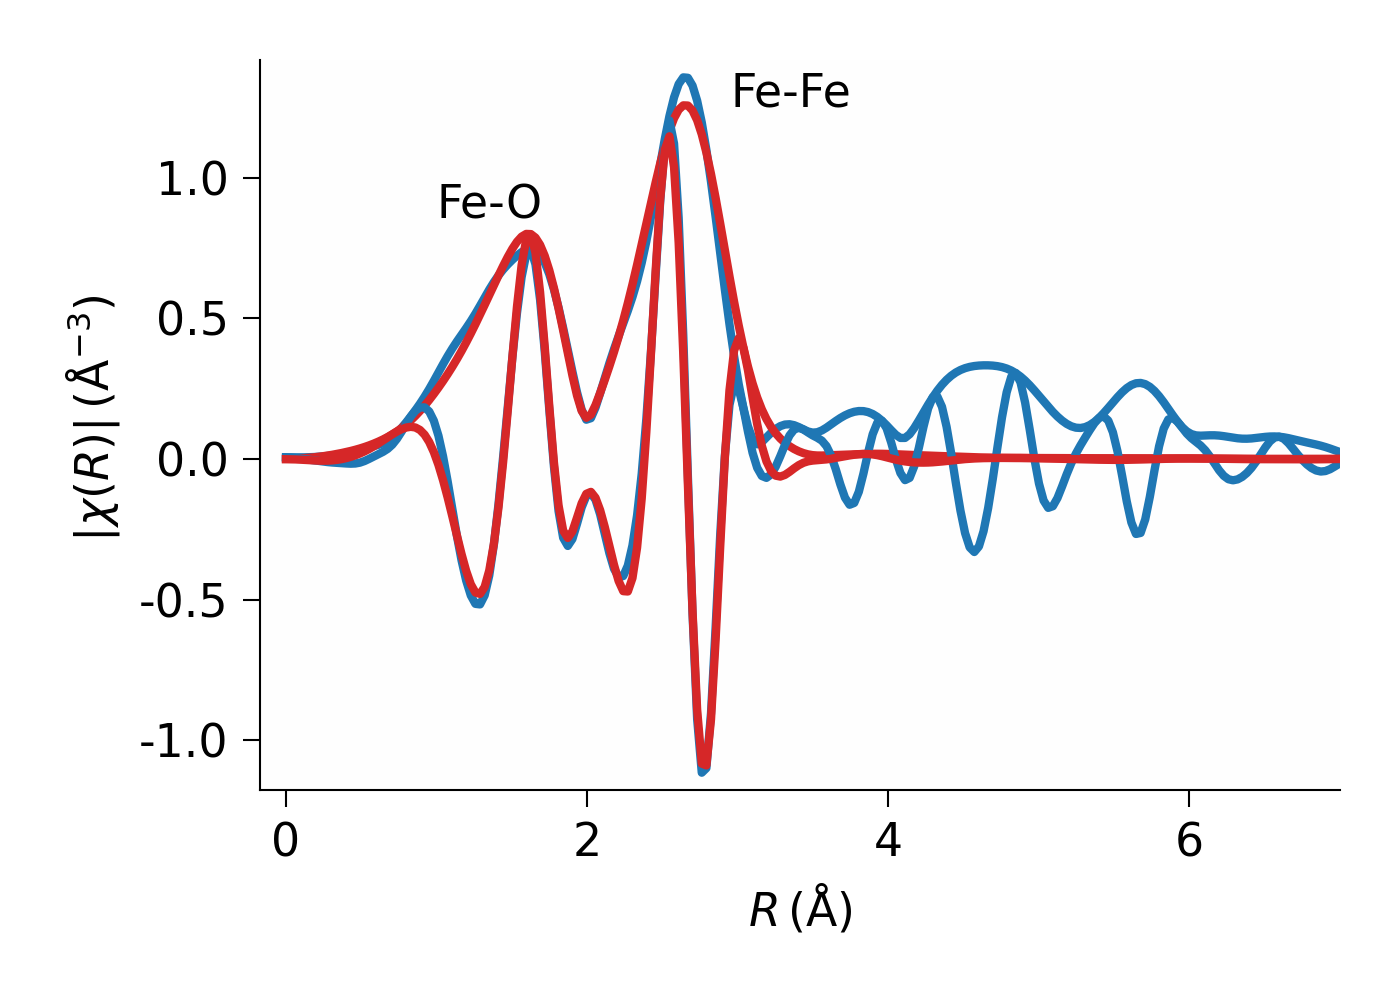
\includegraphics[width=60mm]{figs/fits/feo_2sh_chirre}
      \end{minipage}}
  \end{tabular}

  \end{cenpage}

\vfill
\end{slide}
